\documentclass{article}

\usepackage[utf8]{inputenc}
\usepackage[T1]{fontenc}
\usepackage{times}
\usepackage[cm]{fullpage}
\usepackage[parfill]{parskip}
\usepackage[xindy]{glossaries}
\usepackage[french]{babel}
\usepackage{lmodern}
\usepackage{graphicx}

\graphicspath{{"Diagrammes UML/"}}

\title{Software Requirement Document : Wizard Poker}
\author{Verhelst Théo \and Reynouard Alexis \and Petit Robin \and Muranovic Allan \and Gueniffey Stanislas \and Berrewaerts Jonathan \and Baudoux Nicolas}

% si on ne précise pas le sort explicitement, il n'est pas content... Ça me gonfle donc je laisse comme ça pour l'instant...
% //~ TODO modifier le Sort des 2 derniers selon votre convenance

\newglossaryentry{Duel}{
    type=glossary,
    name={duel},
    description={Affrontement entre deux utilisateurs se solvant en la victoire de l'un des deux joueurs},
    sort=45
}

\newglossaryentry{Facultatif}{
    type=glossary,
    name={facultatif},
    description={Non-requis explicitement ou implicitement par le client mais qui pourra être implémenté par la suite},
    sort=65
}

\newglossaryentry{Deck}{
    type=glossary,
    name={deck},
    description={Paquet d'exactement 20 cartes de jeu ne comprenant pas plus de deux fois la même carte},
    sort=43
}

\newglossaryentry{Fosse}{
    type=glossary,
    name={fosse},
    description={\textit{Pseudo-lieu} du plateau où sont stockées les cartes ayant servi et étant arrivées en fin de vie},
    sort=67
}

\newglossaryentry{Lobby}{
    type=glossary,
    name={lobby},
    description={\textit{Pseudo} salle d'attente où les joueurs patientent le temps que le serveur leur désigne un adversaire},
    sort=125
}

\newglossaryentry{Invoquer}{
    type=glossary,
    name={invoquer},
    description={Utiliser une carte. Consiste à placer un monstre sur le terrain, attquer avec un monstre ou lancer un sort},
    sort=95
}
\newglossaryentry{Creature}{
    type=glossary,
    name={Creature},
    description={Une créature, (ou \textbf{Creature}) est une carte jouable sur le plateau. Elle dispose d'un certain montant de point de vie, d'un coût d'invocation, d'une
    valeur d'attaque et éventuellement d'un ou plusieurs effets, qu'il soit direct ou qu'il applique des contraintes à qui que ce soit.},
    sort=45
}
\newglossaryentry{Sort}{
    type=glossary,
    name={Sort},
    description={Un sort, (ou \textbf{Spell}) est une carte qui déclenche un effet à l'activation. Un sort ne dipose que d'un coût, et d'un ou plusieurs effets.},
    sort=45
},
\newglossaryentry{Pop}{
    type=glossary,
    name={Pop},
    description={Un pop est une action courante sur les piles informatique. Cette action consiste à enelever le sommet de la pile, et à souvent l'utiliser par la même occasion},
    sort=45
},
\newglossaryentry{Push}{
    type=glossary,
    name={Push},
    description={Un push est une action courante sur les piles informatique. Cette action consiste à ajouter un élément au dessus de la pile.},
    sort=45
}



\makeglossary

\begin{document}

\pagenumbering{Roman}
\maketitle
\tableofcontents
\newpage
\pagenumbering{arabic}

\section{Introduction}
    \subsection{But du projet}
        L'objectif visé par ce projet est la réalisation d'une application client-serveur en C/C++. L'application visée est un jeu de carte (appelé
        \textit{Wizard Poker}) tour à tour et multijoueurs en réseau. Elle est destinée à tout type de public, \textit{open source}, libre de droit %licence à définir
        et à but non commercial. C'est un projet académique

        Pour ce faire, notre équipe, composée de sept personnes, dispose de trois phases de développement qui dureront approximativement 4 semaines chacune :
        \begin{itemize}
            \item la première portera uniquement sur la création du squelette respectant toutes les demandes effectuées par les client ;
            \item la deuxième phase concernera l'implémentation en console uniquement ;
            \item et enfin la troisième ajoutera l'interface graphique.
        \end{itemize}

    \subsection{Glossaire}  % doit s'agrandir avec le temps
        \printglossaries

    \subsection{Historique}
        \begin{itemize}
            \item[11/12/2015] réunion et squelette du SRD (équipe) ;
            \item[15/12/2015] création des diagrammes UML (équipe UML) ;  % à expliciter !!
            \item[15/12/2015] rédaction de la version propre du SRD (?).
        \end{itemize}

\section{Besoins de l'utilisateur}
    L'utilisateur de l'application, à savoir le joueur, a un certain nombre de besoins. Ces derniers doivent être satisfaits afin de garantir un confort d'utilisation
    maximal. En utilisant l'application, le joueur \textbf{doit} avoir la possibilité de :

    \begin{itemize}
        \item créer un compte utilisateur ;
        \item créer un \gls{deck} ou en modifier un pré-existant ;
        \item consulter les cartes dont il dispose ;
        \item consulter les \glspl{deck} dont il dispose ;
        \item ajouter un joueur existant en ami ;
        \item discuter avec un ami ;
        \item \textbf{\gls{facultatif} :} discuter avec plusieurs amis simultanément ;
        \item affronter un adversaire aléatoire ;
        \item défier un joueur de sa liste d'amis ;
        \item consulter le classement des joueurs.
    \end{itemize}

    \subsection{Exigences fonctionnelles}
        \subsubsection{Possibilités d'actions de l'utilisateur}
            \begin{center}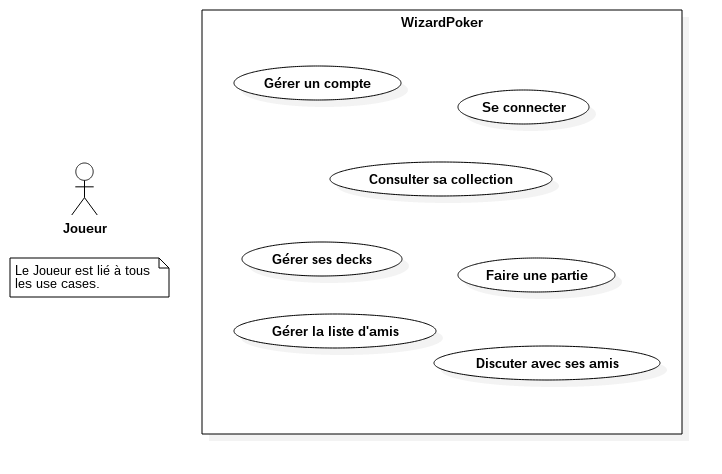
\includegraphics[scale=0.6]{UseCase1_Main.png}\end{center}

        \subsubsection{Création d'un compte}
            \begin{center}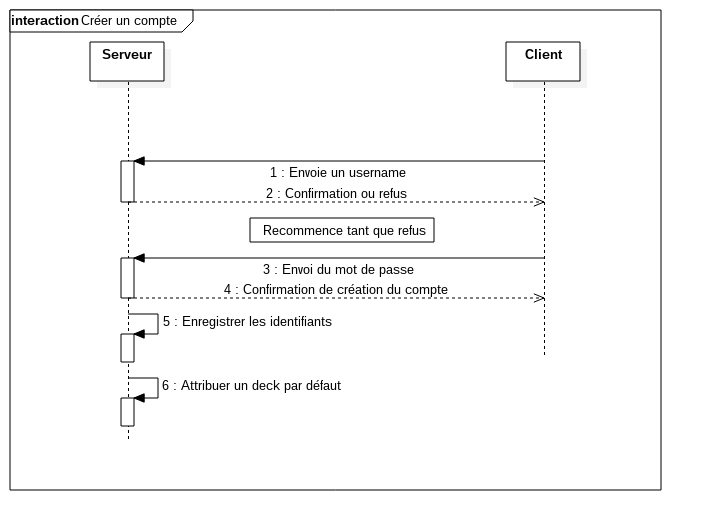
\includegraphics[scale=0.6]{Collaboration1_SignIn.png}\end{center}

            \begin{description}
                \item[Description] L'utilisateur peut créer un compte à l'aide d'un identifiant unique (son pseudo) et d'un mot de passe associé ;
                \item[Pré-condition] l'utilisateur doit être connecté au serveur ;
                \item[Post-condition] Soit la demande est acceptée (identifiant admissible), soit la demande est rejetée (identifiant non-admissible ou déjà utilisé).
            \end{description}

        \subsubsection{Gestion des \glspl{deck}}
            \begin{center}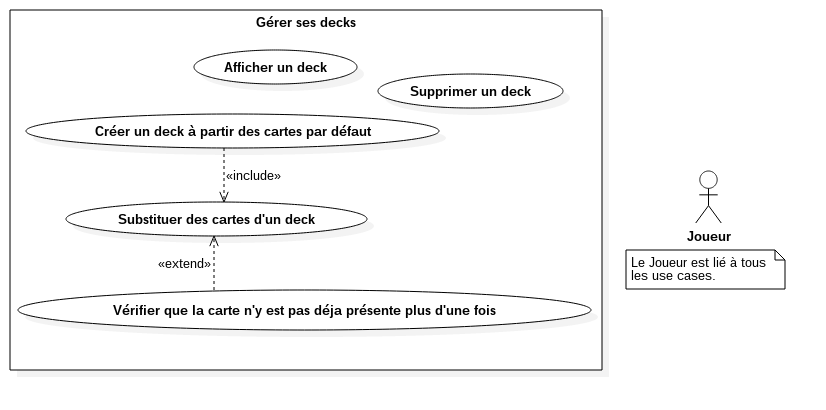
\includegraphics[scale=0.5]{Model1_DecksManagement.png}\end{center}

        \subsubsection{Début de partie}
            \begin{center}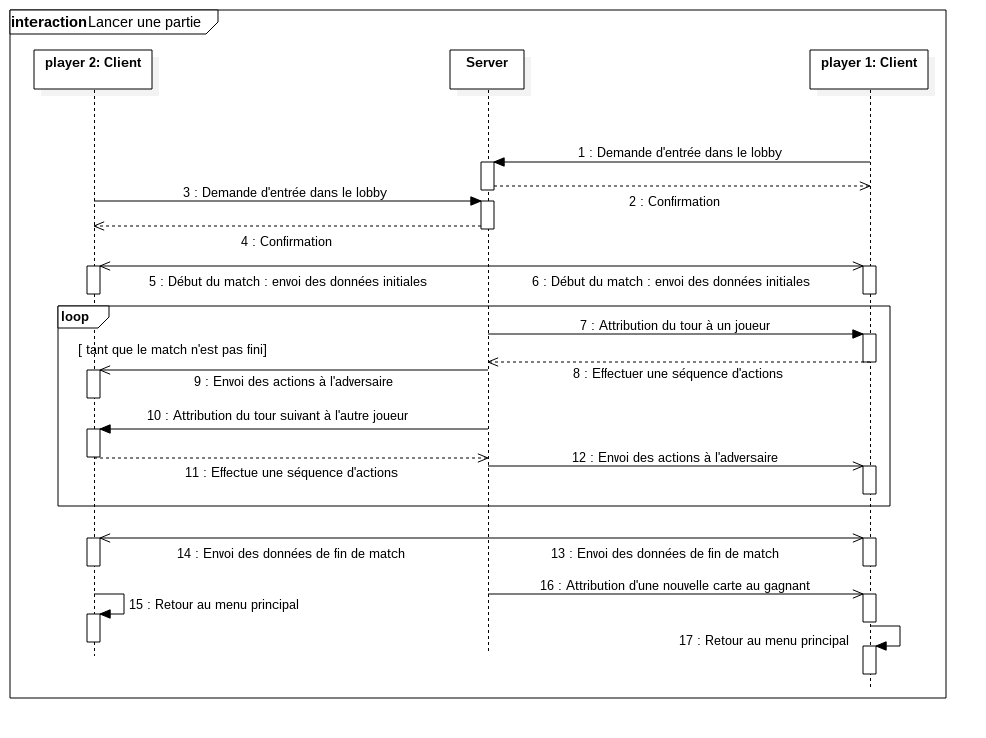
\includegraphics[scale=0.35]{Collaboration2_StartDuel.png}\end{center}

            \begin{description}
                \item[Description] un joueur connecté peut défier un ami ou demander un duel contre un adversaire aléatoire ;
                \item[Pré-condition] chaque utilisateur doit être identifié et connecté à son compte ;
                \item[Post-condition] un joueur aura perdu, l'autre aura gagné\footnote{Le gagnant reçoit une carte aléatoire à ajouter à son \gls{deck}.}.
            \end{description}

    \subsection{Exigences non-fonctionnelles}
        L'application \textbf{doit} tourner sur Linux (salles 008 et 007 du NO.4) et fonctionner en réseau (\textit{a priori} avec clients
        et serveurs sur des machines séparées).

        De plus, l'utilisateur doit pouvoir discuter par messages à n'importe quel moment de l'exécution de l'application : tant pendant
        qu'il gère ses amis, ses cartes ou pendant qu'il est en \gls{duel}. Ces discutions ne peuvent se faire avec un joueur
        n'étant pas ami de l'utilisateur.

    \subsection{Exigences de domaine}
        Les exigences implicites au domaine du jeu sont les suivante :

        \begin{itemize}
            \item l'application doit être accessible à tout utilisateur potentiel ;
            \item l'application doit être \textit{amusante} donc équilibrée ;
            \item \textbf{\gls{facultatif} : } empêcher la triche dans la mesure du possible.
        \end{itemize}

\section{Besoins du système}
    \subsection{Exigences fonctionnelles}
        Dans un premier temps, l'application \textbf{doit} tourner en ligne de commande et doit, dans un second temps adopter une interface
        graphique. De plus, l'application doit être développée en C++.

    \subsection{Exigences non-fonctionnelles}
        Le système \textbf{doit} être maintenable et pensé dans l'optique d'une future adaptation avec interface graphique.

    \subsection{Design et fonctionnement du système}
        La structure du programme est résumée dans les classes suivantes (servant également de \textit{pseudo-squelette de code}) :

        \begin{center}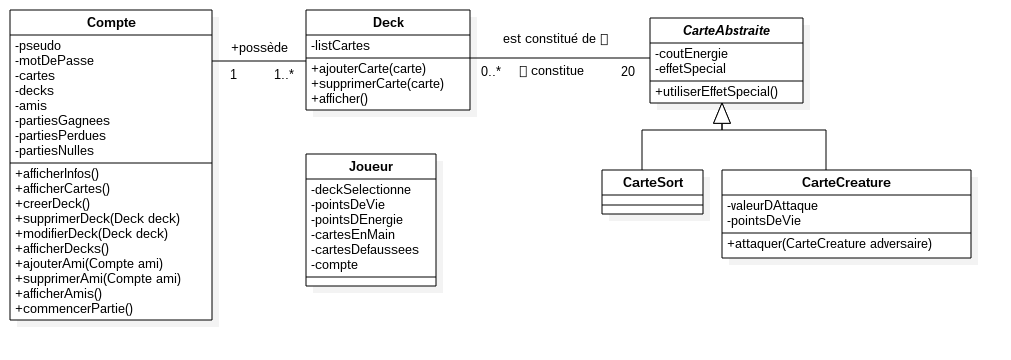
\includegraphics[scale=0.5]{Model2_Classes.png}\end{center}

\section{Index}
    % à générer automatiquement avec LaTeX

\end{document}
